\chapter{Especificación de requerimientos}
\section{Pila de producto}
La plataforma digital para la comunidad de Tejarcillos se ha estructurado mediante un análisis detallado de historias de usuario que permiten visualizar en este informe el MVP 1 del sistema. Para facilitar la trazabilidad y comprensión de la estructura del sistema, se ha implementado una codificación RFXXX (Requerimiento Funcional) para todas las funcionalidades del producto y RNFXXX (Requerimiento No Funcional) para otros requerimientos.

Esta codificación unificada permite mantener una nomenclatura consistente para todos los requerimientos funcionales del sistema, facilitando su identificación, priorización y seguimiento throughout el desarrollo del proyecto.
\subsection{Requerimientos funcionales del sistema}

%% PILA DE PRODUCTO %%
\begin{longtable}{|l||p{7cm}|l|l|}
\multicolumn{4}{c}{Pila general del producto}\\
\hline\hline
\textbf{Código} & \textbf{Descripción} & \textbf{Prioridad} & \textbf{Inserción}\\
\hline
\endfirsthead
\textbf{Código} & \textbf{Descripción} & \textbf{Prioridad} & \textbf{Inserción}\\
\hline\hline
\endhead

\textbf{RF001} & 
\textbf{Implementar sistema de categorías en base de datos:} Creación de una colección de categorías con identificador, nombre y tipo para clasificar contenidos por áreas (arte, cultura, deporte, etc.). La estructura debe permitir ampliaciones futuras y asociación con publicaciones, eventos y emprendimientos. & Alta & Original \\

\textbf{RF002} & 
\textbf{Corrección integral de interfaz de usuario:} Resolución de problemas de navegación, funcionalidad de botones y visualización de información en cards. Incluye agregar botones "Volver", reparar rutas, validar props y asegurar visualización completa de información en eventos y emprendimientos. & Alta & Original \\

\textbf{RF003} & 
\textbf{Sistema de gestión de archivos e imágenes:} Implementación de funcionalidad para subir, almacenar y previsualizar archivos en formatos PNG, JPG y PDF. Incluye servidor confiable para almacenamiento y manejo de errores con mensajes claros para el usuario. & Alta & Original \\

\textbf{RF004} & 
\textbf{API de gestión de categorías backend:} Desarrollo de endpoints RESTful para crear, editar, eliminar y consultar categorías. Incluye validaciones para evitar duplicados y respuestas HTTP consistentes para el frontend. & Alta & Original \\

\textbf{RF005} & 
\textbf{Calendario interactivo de eventos:} Implementación de vista mensual con eventos marcados en sus fechas correspondientes. Incluye endpoint backend para consulta por rangos de fechas y funcionalidad frontend para navegación y visualización de detalles. & Media & Original \\

\textbf{RF006} & 
\textbf{Optimización de biblioteca digital:} Mejora del sistema de carpetas raíz y subcarpetas, verificación de funcionalidad de subida de archivos y optimización de filtros de búsqueda por nombre y tipo de archivo. & Media & Original \\

\textbf{RF007} & 
\textbf{Integración de categorías en frontend:} Implementación de selectores de categoría en formularios de creación y sistema de filtros para visualización de contenidos por área. Inclusión de categorías en cards y vistas detalladas. & Alta & Original \\

\textbf{RNF001} & 
\textbf{Pruebas unitarias en sistema de autenticación y seguridad:} Testeo unitario de flujos de registro, login, logout y recuperación de contraseña. Validación de roles de usuario, seguridad en credenciales y funcionamiento correcto en todos los módulos. & Media & Original \\

\color{Mahogany}
\textbf{RNF002} & 
\textbf{Pruebas integrales y control de calidad:} Revisión completa de todos los flujos principales del sistema, corrección de errores menores y validación de cumplimiento de requisitos del cliente. Pruebas de regresión previas a la entrega. & Alta & \textbf{Eliminado} \\

\color{ForestGreen}
\textbf{RF008} & 
\textbf{Subir archivos a biblioteca:} Permitir la subida y almacenamiento de archivos (no imágenes) en la biblioteca; se creó como división de RF003. & Alta & Añadido  \\

\color{ForestGreen}
\textbf{RF009} & 
\textbf{Corrección y ampliación de campos en publicaciones:} Asegurar persistencia de campos adicionales (precio, horaEvento) en BD y correcta visualización en vistas; surgió por pruebas del calendario. & Media & Añadido  \\

\color{ForestGreen}
\textbf{RF010} & 
\textbf{Adaptación responsive y manejo de errores:} Implementación de responsive para todas las vistas, validaciones y mensajes de error en subida de archivos y mostrar la hora en la agenda. & Media & Añadido \\

\hline
\caption{\color{ForestGreen}VERDE: Historias agregadas en esta iteración. \color{Mahogany}ROJO: Historias eliminadas.}
\label{ProductBacklog}
\end{longtable}


\subsection{Bitácora de cambios}
\begin{itemize}
    \item \textbf{División de RF003 (04/09):}  
    El requerimiento RF003 - Subir imágenes y archivos al servidor fue dividido, originalmente valía 2 puntos. Se dejó el RF003 únicamente para subir imágenes al servidor (1 punto) y se creó el nuevo requerimiento RF008 - Subir archivos a biblioteca (1 punto), debido a que ambas tareas eran independientes y en un inicio se asumió que los archivos e imagenes se guardaban en el servidor Digital Ocean, pero al revisar bien el código no era así como estaba la cofiguración en el proyecto, en este requerimiento (FR008) los archivos se guardan en la base de datos, mientras que las imágenes se guardan en Digital Ocean.
   
    \item \textbf{Creación de RF009 (09/09):}  
    Durante la integración del calendario y las publicaciones se detectaron campos faltantes (\textit{precio}, \textit{horaEvento}) que requerían persistencia en la base de datos y ajustes en las vistas.  
    Se creó RF009 (3 puntos) para asegurar la persistencia y la correcta visualización. RF009 fue aceptado en el sprint y luego completado.

    \item \textbf{Creación de RF010 y eliminación de RNF002 (16/09):}  
    Se acordó añadir RF010 (Adaptación responsive y manejo de errores - 3 puntos) para cubrir trabajo crítico de adaptación a dispositivos, ya que inicialmente en la vista móvil existían elementos superpuestos.
    Dado que en RF010 se abarcó pruebas funcionales que se pretendían cubrir con RNF002, se decidió eliminar RNF002 por redundancia.
    RNF002 se marcó como eliminado porque su \textit{scope} fue absorbido por RF010.
\end{itemize}

\section{Producto Mínimo Viable de la iteración 1}
El MVP del Sprint 1 se centra en mejorar y estabilizar la plataforma existente para la comunidad de Tejarcillos, trabajando sobre la base ya desarrollada para corregir problemas críticos y agregar funcionalidades esenciales que permitan su uso efectivo por parte de los usuarios.

Este primer producto mínimo viable se enfoca en las siguientes áreas de mejora:

\begin{itemize}
\item \textbf{Corrección de problemas en publicaciones y eventos}: Resolución de errores críticos en los módulos existentes de publicaciones y eventos, asegurando que toda la información se muestre correctamente, los botones funcionen adecuadamente y la navegación sea fluida y sin interrupciones.

\item \textbf{Implementación de sistema de categorías}: Adición de categorías para organizar y clasificar los contenidos por áreas temáticas (arte, cultura, deporte, educación), permitiendo búsquedas y filtros más eficientes tanto en publicaciones como en eventos.

\item \textbf{Calendarización de eventos}: Desarrollo de un calendario interactivo que muestre los eventos programados, facilitando la visualización de la agenda comunitaria y el acceso a información detallada de cada actividad.

\item \textbf{Incorporación de servidor para archivos}: Integración del sistema de subida y almacenamiento de imágenes y archivos para publicaciones y eventos, asegurando que funcione de manera confiable.

\item \textbf{Verificación de funcionalidades básicas}: Testeo integral del sistema de login, registro y navegación para garantizar que todas las funcionalidades centrales operen correctamente.

\item \textbf{Pruebas de estabilidad}: Validación completa de que la plataforma funciona sin errores críticos y está lista para su uso por la comunidad.
\end{itemize}
Al finalizar este sprint, la plataforma estará operativa, estable y organizada, permitiendo a los usuarios de Tejarcillos publicar contenidos, visualizar eventos en el calendario y navegar de manera intuitiva por las diferentes categorías de interés comunitario.

\subsection{Pila de trabajo de la iteración 1}

El equipo de desarrollo está compuesto por tres integrantes con dedicación de 12 horas semanales cada uno trabajando durante 4 semanas (20 días hábiles), totalizando 144 horas de capacidad al 100\%. Considerando un factor de productividad del 90\% para imprevistos y reuniones de coordinación, el presupuesto disponible es de 128 horas equivalentes a 32 puntos de historia para el Sprint 1.

\begin{longtable}{|l|l|l|}
    \hline
    \textbf{Miembro del equipo} & \textbf{Rol} & \textbf{Capacidad (puntos)} \\
    \hline
    Fredrik Aburto Jiménez & Desarrollo Fullstack & 12 \\
    Angélica Díaz Barrios & Desarrollo Fullstack & 12 \\
    Andrés Salas Araya & Desarrollo Fullstack & 12 \\
    \hline\hline
    \textbf{Presupuesto total (100\%):} & & 36\\
    \textbf{Presupuesto disponible (90\%):} & & 32\\
    \textbf{Presupuesto en horas al 90\% (1 punto = 4 horas):} &  & 128\\
    \hline
    \caption{Resumen de capacidad de carga del equipo para la iteración 1}
\end{longtable}

%% PILA DEL SPRINT (ITERACIÓN) %%
\begin{longtable}{|l||c|c|p{7cm}|l|}
\multicolumn{5}{c}{Pila de la \textbf{iteración 1}} \\
\hline\hline
\textbf{Código} & \textbf{CE} & \textbf{CR} & \textbf{Responsables} & \textbf{Finalización} \\
\hline
\endfirsthead
\textbf{Código} & \textbf{CE} & \textbf{CR} & \textbf{Responsables} & \textbf{Finalización} \\
\hline\hline
\endhead

\textbf{RF001} & 1 & 1 & Angélica Díaz Barrios & 01/09/2025 \\

\textbf{RF002} & 3 & 2 & Fredrik Aburto Jiménez & 18/09/2025 \\

\textbf{RF003} & 2 & 2 & Andrés Salas Araya & 04/09/2025 \\

\textbf{RF004} & 2 & 2 & Angélica Díaz Barrios & 02/09/2025 \\

\textbf{RF005} & 3 & 2 & Angélica Díaz Barrios & 09/09/2025 \\

\textbf{RF006} & 1 & 2 & Fredrik Aburto Jiménez & 04/09/2025 \\

\textbf{RF007} & 2 & 3 & Angélica Díaz Barrios & 11/09/2025 \\

\textbf{RNF001} & 1 & 2 & Fredrik Aburto Jiménez & 11/09/2025 \\

\textcolor{red}{\textbf{RNF002}} & 1 & 0 & \textcolor{red}{N/A} & \textcolor{red}{N/A} \\

\textcolor{ForestGreen}{\textbf{RF008}} & 0 & 2 & Andrés Salas Araya & 12/09/2025 \\

\textcolor{ForestGreen}{\textbf{RF009}} & 0 & 2 & Andrés Salas Araya & 15/09/2025 \\

\textcolor{ForestGreen}{\textbf{RF010}} & 0 & 1 & Angélica Díaz Barrios & 22/09/2025 \\
\hline
\textbf{Total} & \textbf{16} & \textbf{21} & & \\
\hline

\caption{Pila de la Iteración 1. \textbf{CE:} Carga Estimada, \textbf{CR:} Carga Real (redondeada a puntos).}
\label{SprintBacklog}
\end{longtable}


\subsection{Desempeño del equipo}

Durante el desarrollo de la iteración se presentaron algunas situaciones que llevaron a ajustes en la pila de trabajo planificada:

\begin{itemize}
    \item El requerimiento \textbf{RF003} (Subir imágenes y archivos al servidor), estimado originalmente en 2 puntos, se dividió en dos tareas independientes: \textbf{RF003} (Subir imágenes) y \textbf{RF008} (Subir archivos a la biblioteca). Esta decisión se tomó porque ambas actividades eran técnicamente separables y tenían entregables distintos. Aunque se dividió en 1 punto para cada tarea, estas requirieron 2 puntos cada una para completarse, por lo que aquí podemos ver que se dió una subestimación para ambas tareas, no se tomó en cuenta su complejidad.
    \item Derivado de la integración del calendario interactivo, surgió el nuevo requerimiento \textbf{RF009} (Corrección y ampliación de campos en publicaciones), ya que los nuevos atributos \texttt{precio} y \texttt{horaEvento} no se estaban almacenando en la base de datos. El campo precio sí se solicitaba en el formulario, pero no se guaradaba en la base de datos y el campo de hora evento se incoorporó ya que se consideraba necesario para los eventos.
    \item Hacia el cierre del sprint, se creó el requerimiento \textbf{RF010} (Adaptación responsive y manejo de errores), con el fin de mejorar la presentación y estabilidad de la aplicación antes de entregar el MVP.
    \item El requerimiento \textbf{RNF002}, inicialmente contemplado, no se ejecutó dentro de este sprint, ya que se habían realizado pruebas unitarias previamente en otros requerimientos.
\end{itemize}

A pesar de estas modificaciones, la coordinación del equipo permitió completar los requerimientos planificados y los nuevos que surgieron durante la ejecución.

En cuanto al presupuesto y la velocidad del equipo, los resultados fueron los siguientes:

\begin{itemize}
    \item \textbf{Carga estimada total:} 16 puntos (64 horas).
    \item \textbf{Carga real total:} 21 puntos (84 horas).
    \item \textbf{Velocidad del equipo:} 21 puntos en el Sprint 1.
\end{itemize}

La velocidad individual de cada integrante fue:

\begin{itemize}
    \item \textbf{Angélica Díaz Barrios:} 1 + 2 + 2 + 3 + 1 = \textbf{9 puntos}.
    \item \textbf{Fredrik Aburto Jiménez:} 2 + 2 + 2 = \textbf{6 puntos}.
    \item \textbf{Andrés Salas Araya:} 2 + 2 + 2 = \textbf{6 puntos}.
\end{itemize}


\bigskip

\subsubsection*{Diferencias entre carga estimada y real}

\begin{itemize}
    \item \textbf{Diferencia:} $21 - 16 = 5$ puntos adicionales.
    \item \textbf{Porcentaje de sobrecarga:} $\dfrac{CR - CE}{CE} \times 100 = \dfrac{21 - 16}{16} \times 100 \approx 31.25\%$.
\end{itemize}

Esto muestra que existió una \textbf{subestimación} en la planificación inicial, ya que el equipo terminó ejecutando aproximadamente un 31\% más de carga de la prevista. La principal causa fue la aparición de requerimientos no identificados al inicio (\textbf{RF008}, \textbf{RF009} y \textbf{RF010}), los cuales incrementaron la carga real sin estar contemplados en la estimación original.

\bigskip

\subsubsection*{Requerimientos sobreestimados y subestimados}

\begin{itemize}
    \item \textbf{Sobreestimados:}
        \begin{itemize}
            \item \textbf{RF002:} Estimado en 3, requirió 2.
            \item \textbf{RF005:} Estimado en 3, requirió 2.
        \end{itemize}

    \item \textbf{Subestimados:}
        \begin{itemize}
            \item \textbf{RF006:} Estimado en 1, requirió 2.
            \item \textbf{RF007:} Estimado en 2, requirió 3.
            \item \textbf{RF003 + RF008:} Originalmente estimado en 2, pero dividido en dos requerimientos que terminaron sumando 4 puntos reales (subestimación por complejidad técnica).
            \item \textbf{RNF001:} Estimado en 1, requirió 2.
        \end{itemize}
\end{itemize}

\bigskip

La siguiente gráfica de quemado (véase Figura~\ref{fig:grafica_quemado}) refleja el avance acumulado del sprint con respecto a la carga estimada:

\begin{table}[H]
\centering
\begin{tabular}{|c|c|c|}
\hline
\textbf{Día} & \textbf{Tendencia} & \textbf{Real} \\ \hline
0  & 16   & 21 \\ \hline
1  & 15,2 & 20 \\ \hline
2  & 14,4 & 18 \\ \hline
3  & 13,6 & 18 \\ \hline
4  & 12,8 & 14 \\ \hline
5  & 12   & 14 \\ \hline
6  & 11,2 & 14 \\ \hline
7  & 10,4 & 12 \\ \hline
8  & 9,6  & 12 \\ \hline
9  & 8,8  & 7  \\ \hline
10 & 8    & 5  \\ \hline
11 & 7,2  & 3  \\ \hline
12 & 6,4  & 3  \\ \hline
13 & 5,6  & 3  \\ \hline
14 & 4,8  & 1  \\ \hline
15 & 4,0  & 1  \\ \hline
16 & 3,2  & 0  \\ \hline
17 & 2,4  &    \\ \hline
18 & 1,6  &    \\ \hline
19 & 0,8  &    \\ \hline
20 & -5,10703E-15 & \\ \hline
\end{tabular}
\caption{Tabla de referencia utilizada para el cálculo de la gráfica de quemado del Sprint 1.}
\end{table}

% Gráfica de quemado
\begin{figure}[H]
  \centering
    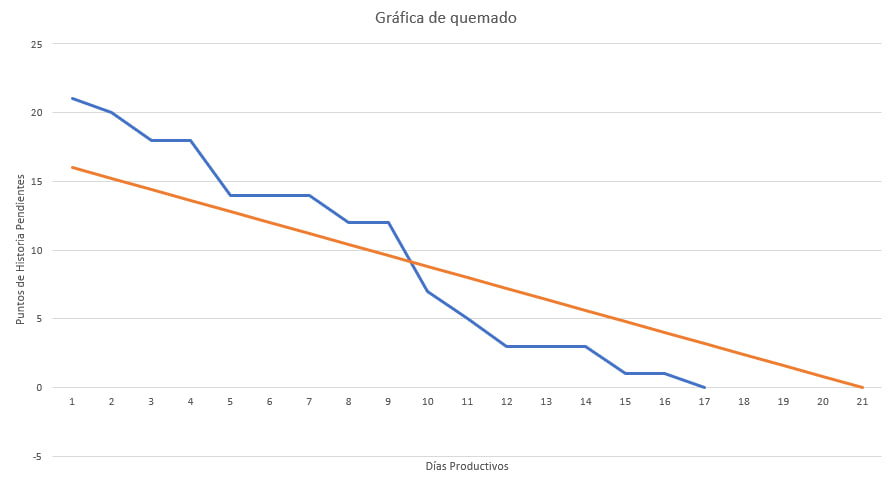
\includegraphics[height=10cm, width=15cm]{project/images/grafica.jpg}
  \caption{Gráfica de quemado del Sprint 1.}
  \label{fig:grafica_quemado}
\end{figure}

